\documentclass{beamer}

\usepackage[russian]{babel}
\usepackage[utf8]{inputenc}
\usepackage{cmap}
\usepackage{graphicx}
\usepackage{xspace}
\usepackage{psfrag}
\usepackage{float}

\newcommand{\MARK}[1]{{\bf {\it #1}}}
\newcommand{\CODE}[1]{{\ttfamily #1}}

\setbeamertemplate{footline}[frame number]
\usecolortheme{seahorse}
\beamertemplateshadingbackground{white}{blue!3}

\begin{document}

\begin{frame}
\begin{center}
БАКАЛАВРСКАЯ РАБОТА\\
\vspace{1cm}
{ СОЗДАНИЕ ИНСТРУМЕНТАРИЯ ДЛЯ ТЕСТИРОВАНИЯ ЦЕЛОСТНОСТИ РЕПОЗИТОРИЯ ПАКЕТНОГО МЕНЕДЖЕРА DEEPSOLVER}
\\
направление подготовки
«Информационные технологии»
\end{center}
\begin{tabbing}
\hspace{6.5cm} \= Исполнитель:\\
\> Кирюшкина В. Е.\\
\vspace{0.5cm}
\hspace{6.5cm} \= Научный руководитель:\\
\> Пожидаев М. С.\\
\end{tabbing}
\end{frame}

\begin{frame}
\frametitle{Дистрибуция ПО в Linux}
\textbf{Репозиторий} - централизованное хранилище программ в сети.\\
\vspace{0.5cm}
Основное свойство репозитория - целостность.\\
\vspace{0.5cm}
Программа --- \textbf{пакет}. Пакеты тесно связаны друг с другом.

\end{frame}

\begin{frame}
\frametitle{Deepsolver}
\textbf{Deepsolver} - система управления пакетами (пакетный менеджер) от \textit{ALT Linux}.\\
\vspace{0.5cm}
Проблема: необходимо осуществлять контроль целостности репозитория \textit{Deepsolver}. 

\end{frame}

\begin{frame}
\frametitle{Цель работы}
Цель настоящей работы:\\
Создание  программного 
продукта, проверяющего целостностноть репозитория Deepsolver.

\end{frame}

\begin{frame}
\frametitle{Зависимости между пакетами}
\begin{itemize}
\item
\textit{provide}: пакет предоставляет функциональность другого пакета. Неявный
provide - имя пакета;
\item
\textit{requires}: пакет требует обязательное наличие другого пакета, указанного 
по его имени или по одному из его provides;
\item
\textit{conflicts}: пакет запрещает наличие другого пакета, указанного по его имени 
или по provides;
\item 
\textit{obsoletes}: пакет может указывать, что является обновлением некоторого 
множества пакетов. 
\end{itemize}

\end{frame}

\begin{frame}
\frametitle{Репозиторий пакетного менеджера Deepsolver}
\begin{itemize}
\item
В репозитории около 60 000 пакетов
\item
Каждый пакет в среднем содержит 9 require и 2 provide
\end{itemize}

Следствие: удаление и добавление пакетов с учетом зависимостей ---
нетривиальная задача.\\

Изменения отражаются в метаданных репозитория - индексе.
\end{frame}

\begin{frame}
\frametitle{Изменение индекса в Deepsolver}
Механизм обновления индекса внутри атвоматизированной части  \textit{Deepsolver}.\\
\vspace{0.5cm}
Задача механизма: обеспечение целостности при внесении изменений в индекс.\\
\vspace{0.5cm}
Для обеспечения целостности - контроль работы механизма.

\end{frame}

\begin{frame}
\frametitle{Цель работы}
Цель работы:
\begin{itemize}
\item
Создание утилиты для проверки готового индекса.
\item
Тестирование утилит для обновления индекса.
\end{itemize}
\vspace{0.5cm}
Часть проверки: отслеживание появления
неактуальных данных, засчет которых неоправданно увеличивается размер индекса.
\end{frame}

\begin{frame}
\frametitle{Индекс репозитория Deepsolver}
\begin{itemize}
\item
Индекс хранится на ftp-сервер ALT Linux.
\item
Индекс - набор файлов с информацией о пакетах репозитория различной детализации.
\item
Свой набор файлов для каждой архитектуры.
\end{itemize}
\end{frame}

\begin{frame}
\frametitle{Условия целостности репозитория}
Условия целостности репозитория:
\begin{itemize}
\item{Для каждого \textit{require} пакета существует одноименный \textit{provide} 
другого пакета.}
\item{Для каждого \textit{provide} существует одноименный \textit{require/conflict} или
он находится в директории из заранее заданного списка.}
\item{Для каждого \textit{conflict} пакета существует одноименный \textit{provide}
другого пакета.}
\end{itemize}
\end{frame}

\begin{frame}
\frametitle{Нарушение условий целостности}
Виды ошибок при нарушении условий целостности:
\begin{itemize}
\item
Анмет - \textit{require} без соответствующего \textit{provide};
\item
Избыточный \textit{provide} - \textit{provide} без соответствующего \textit{require/conflict}
\item
``Избыточный'' \textit{conflict} - \textit{conflict} без соответсвующего \textit{provide}
\end{itemize}
\end{frame}

\begin{frame}
\frametitle{Утилита для проверки готового индекса}
\textbf{Входные данные}: индекс-файл, содержащий основной
список пакетов с информацией о 
зависимостях между ними.\\

\vspace{1cm}

\textbf{Выходные данные}: статистика о наденных ошибках.\\
\end{frame}

\begin{frame}
\frametitle{Статистика}
Формат статистики:\\
\vspace{0.5cm}
Found [количество найденных пакетов] packages\\
.[количество поврежденных пакетов] packages are damaged\\
.[количество пакетов с избыточными provide] packages have unmatched provides\\
.[количество пакетов с анметами] packages have unmets\\
.[количество пакетов с избыточными conflict] packages have unmatched conflicts\\

\end{frame}

\begin{frame}
\frametitle{Диаграмма классов основного модуля}

\begin{figure}
\begin{center}
\vspace{0cm}
\hspace*{-1cm} 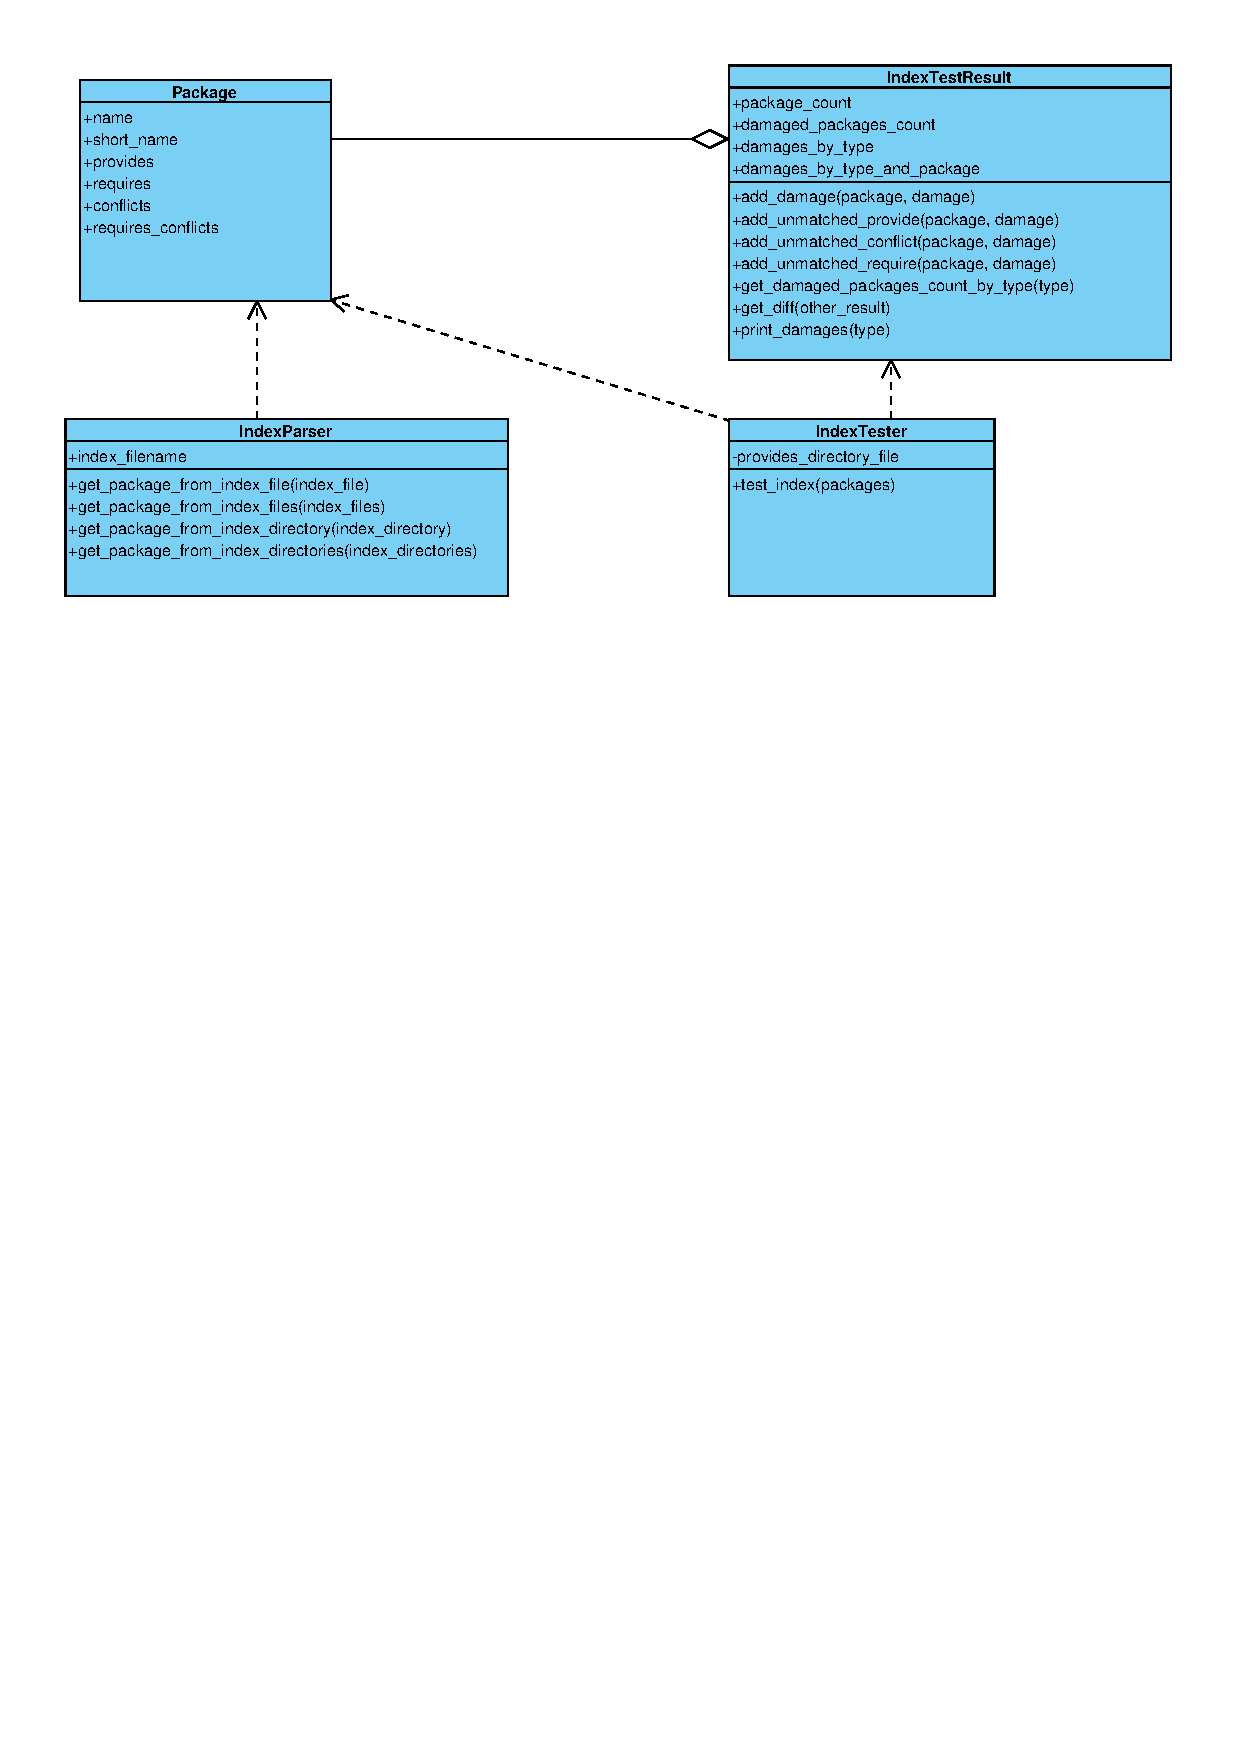
\includegraphics[scale=0.6]{../resources/uml/ds_test_class_diagram.pdf}
\end{center}
\end{figure}

\end{frame}

\begin{frame}
\frametitle{Диаграмма последовательности для алгоритма проверки индекса.}
\subsubsection{Детали реализации}
\begin{figure}
\begin{center}
\vspace{0cm}
\hspace*{-1cm}
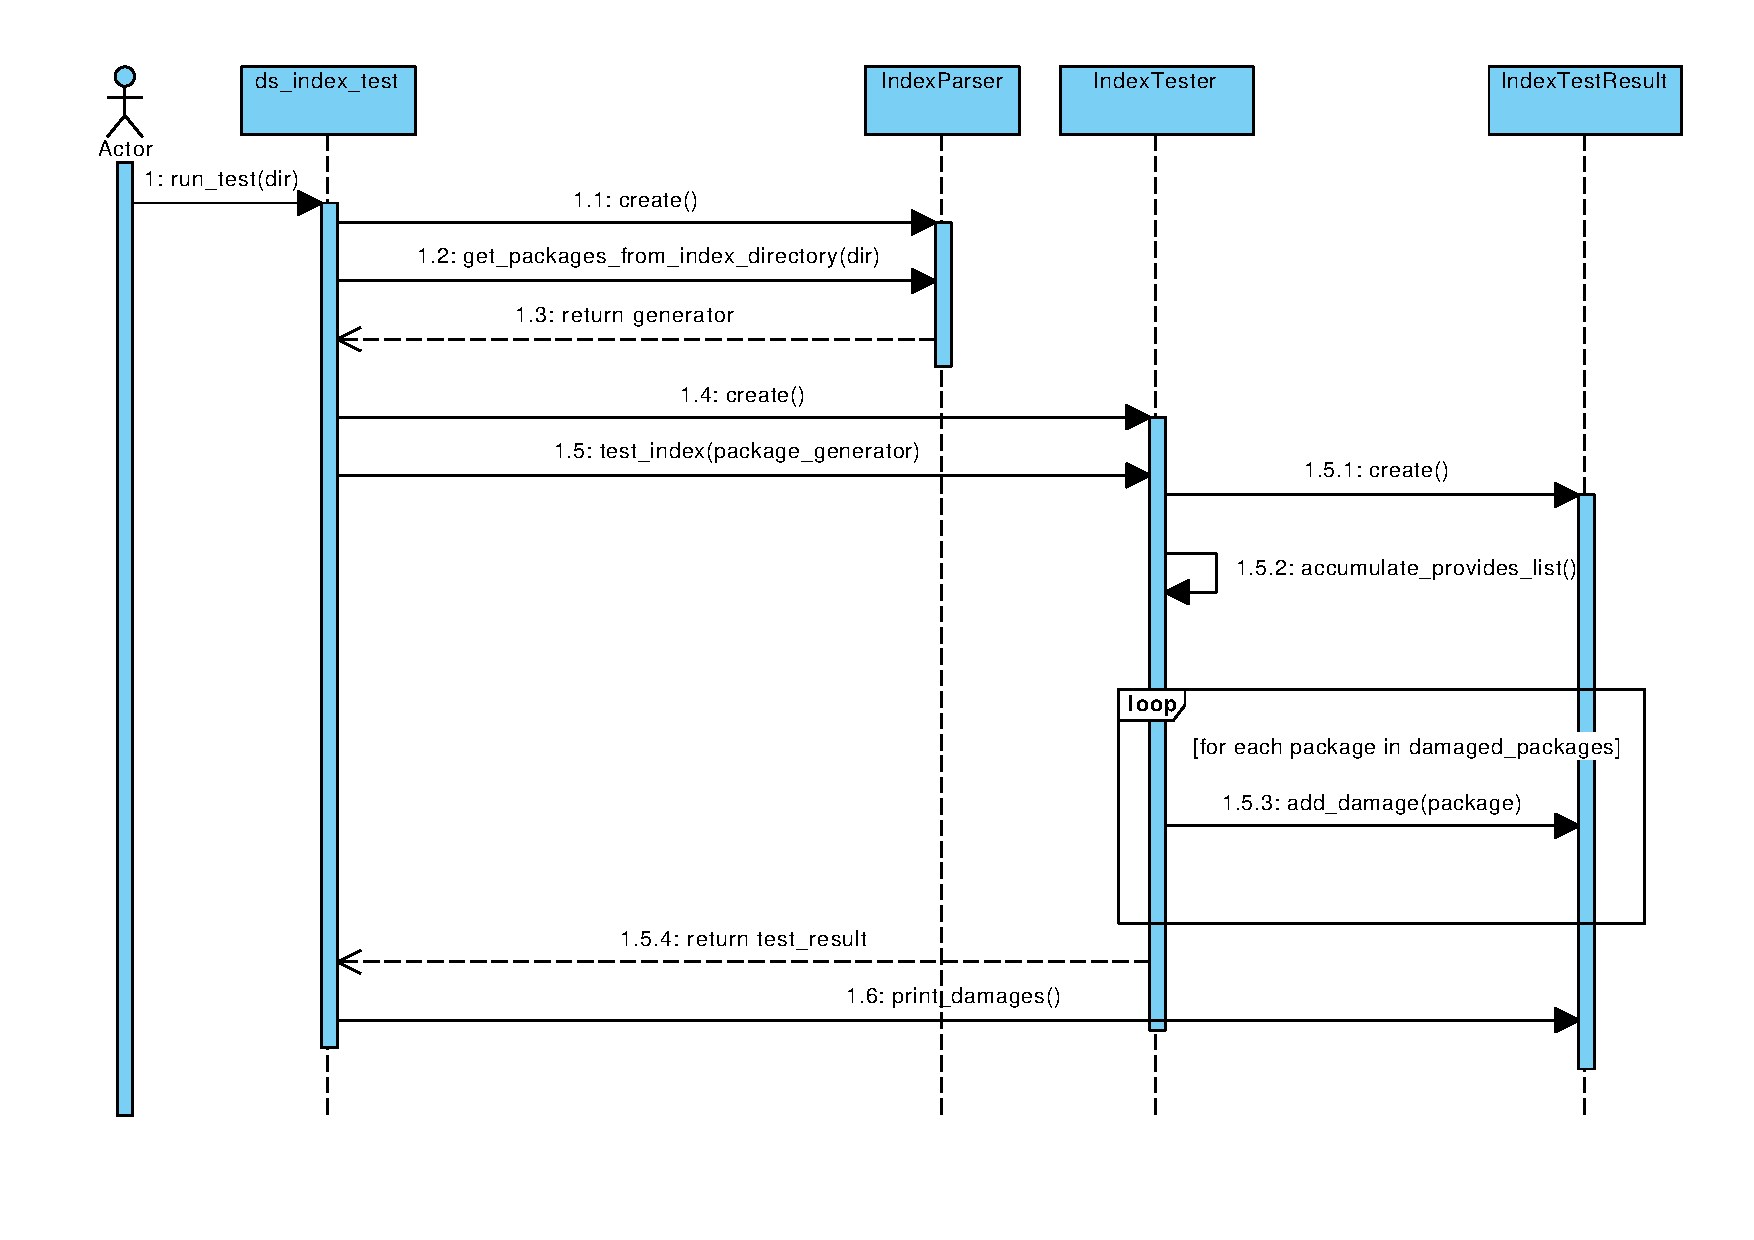
\includegraphics[scale=0.4, clip]{../resources/uml/SimpleTestCase.pdf}
\end{center}
\end{figure}
\end{frame}


\begin{frame}
\frametitle{Утилита для проверки механизма обновления индекса}
\textbf{Входные данные}: весь набор индекс-файлов для данной архитектуры.\\
\vspace{0.5cm}
Этапы проверки:
\begin{itemize}
\item
проверка на неизмененном индексе;
\item
проверка индекса после каждого запуcка механизма обновления.
\end{itemize}
\textbf{Выходные данные}: статистика о найденных ошибках на неизменнои индексе
и после каждого обновления.
\end{frame}

\begin{frame}
\frametitle{Результаты}
Созданы:
\begin{itemize}
\item
утилита для проверки готового индекса;
\item
утилита для проверки механизма обновления индекса
\end{itemize}


Разработанные утилиты применялись для решения промышленных задач:
\begin{itemize}
\item
Активно использовались на стадии отладки процедуры обновления индекса репозитория \textit{Deepsolver}.
\item
Производилась проверка целостности индексов репозитория \textit{Deepsolver} после интеграции в официальный репозиторий
\textit{ALT Linux}.

\end{itemize}
\end{frame}

\begin{frame}
{\Large Спасибо за внимание!}
\end{frame}

\end{document}
